\documentclass{article}

% Language setting
% Replace `english' with e.g. `spanish' to change the document language
\usepackage[english]{babel}

% Set page size and margins
% Replace `letterpaper' with `a4paper' for UK/EU standard size
\usepackage[letterpaper,top=2cm,bottom=2cm,left=3cm,right=3cm,marginparwidth=1.75cm]{geometry}

% Useful packages
\usepackage{amsmath}
\usepackage{amssymb}
\usepackage{graphicx}
\usepackage{inconsolata}
\usepackage{minted}
\usepackage[colorlinks=true, allcolors=blue]{hyperref}

\title{R2 Eksamen}
\author{Skrevet av André Hansen}

\begin{document}
\maketitle

\begin{abstract}
Dette er en template til selve eksamen
\end{abstract}

\section{Del 1: Uten hjelpemidler}

\subsection{Oppgave 2: Oppgi de nøaktige verdiene}

\subsubsection{$tan 45^{\circ}$}

$$\tan 45^{\circ} = 1$$

\subsubsection{$sin 120^{\circ}$}

$$\sin 120^{\circ} = \frac{\sqrt{3}}{2}$$

Oppgave med bilde

\subsection{Oppgave 5: Gitt funksjonen $f(x)=2sin(\frac{x}{2}+\frac{\pi}{4})-1, \quad x \in [-4\pi, 4\pi)$}

\subsubsection{hva er nullpunktene til $f(x)$}

\begin{align*}
    f(x) &= 0 \\
    2\sin(\frac{x}{2}+\frac{\pi}{4})-1 &= 0 , \quad x \in [-4\pi, 4\pi)  \\
    2\sin(\frac{x}{2}+\frac{\pi}{4}) &= 1 \\
    \sin(\frac{x}{2}+\frac{\pi}{4}) &= \frac{1}{2} \\
    \frac{x}{2} + \frac{\pi}{4} = \frac{\pi}{6} + 2\pi \cdot k  & \lor \frac{x}{2} + \frac{\pi}{2} = \frac{\pi}{6} \cdot 2\pi \cdot k, \quad k\in\mathbb{Z} \\
    x+\pi=\frac{\pi}{3} + 4\pi \cdot k &\lor x + \pi = \frac{\pi}{3} + 4\pi \cdot k \\
    x=-\frac{2\pi}{3} \cdot 4\pi \cdot k & \lor  x=\frac{4\pi}{3} + 4\pi \cdot k \\
    x=-\frac{2\pi}{3} + 4\pi \cdot k & \lor  x=\frac{4\pi}{3} + 4\pi \cdot k, \quad k \in \{ -1, 0, 1\} \\
    L= \{-\frac{8\pi}{3}, -\frac{2\pi}{3}, & \frac{4\pi}{3}, \frac{10\pi}{3} \}
\end{align*}

\subsubsection{Skiser grafen}

\begin{figure}[h]
    \centering
    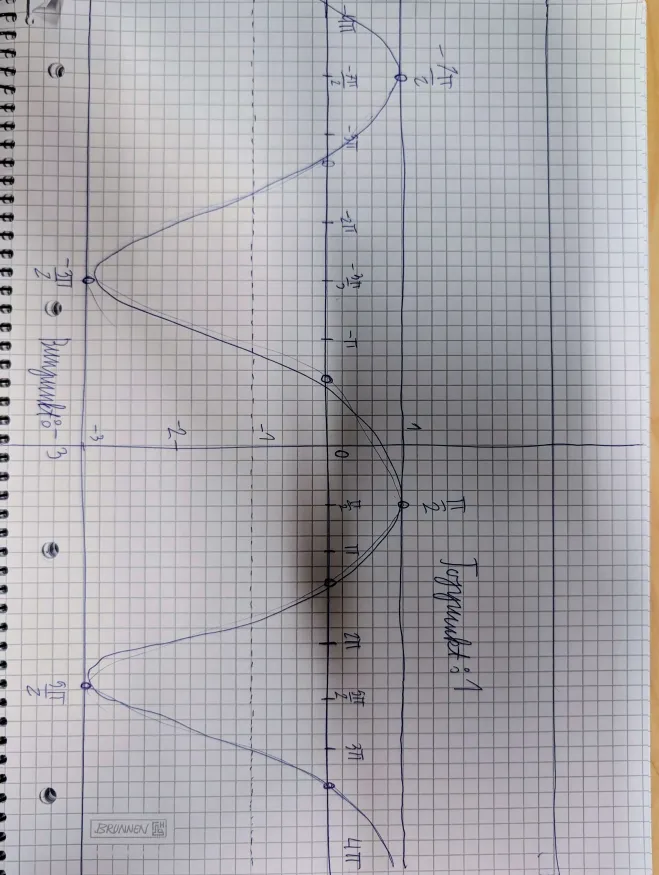
\includegraphics[width=0.7\textwidth, angle=90]{tegning.png}
    \caption{Skisse av grafen}
\end{figure}

\section{Del 2: Med hjelpemidler}

\bibliographystyle{alpha}
\bibliography{sample}

\end{document}
